\section{AtCoder}

\ptitle{[AGC035C] Skolem XOR Tree}{pufanyi}

\prob 给 $n\ (n\le 10^5)$ 个白点 $n$ 个黑点,标号分别为 $1\sim n$。现在需要把这 $2n$ 个点连成一棵树,使得编号为 $i$ 的白点和黑点路径的 xor 和为 $i$。有可能无解。
\sol 如果 $n=2^k$,我们发现第 $n$ 个白点和黑点路径 xor 和的第 $k$ 位肯定是 $0$,那无解。

如果 $n$ 是奇数,我们考虑这样构造:

\begin{center}
    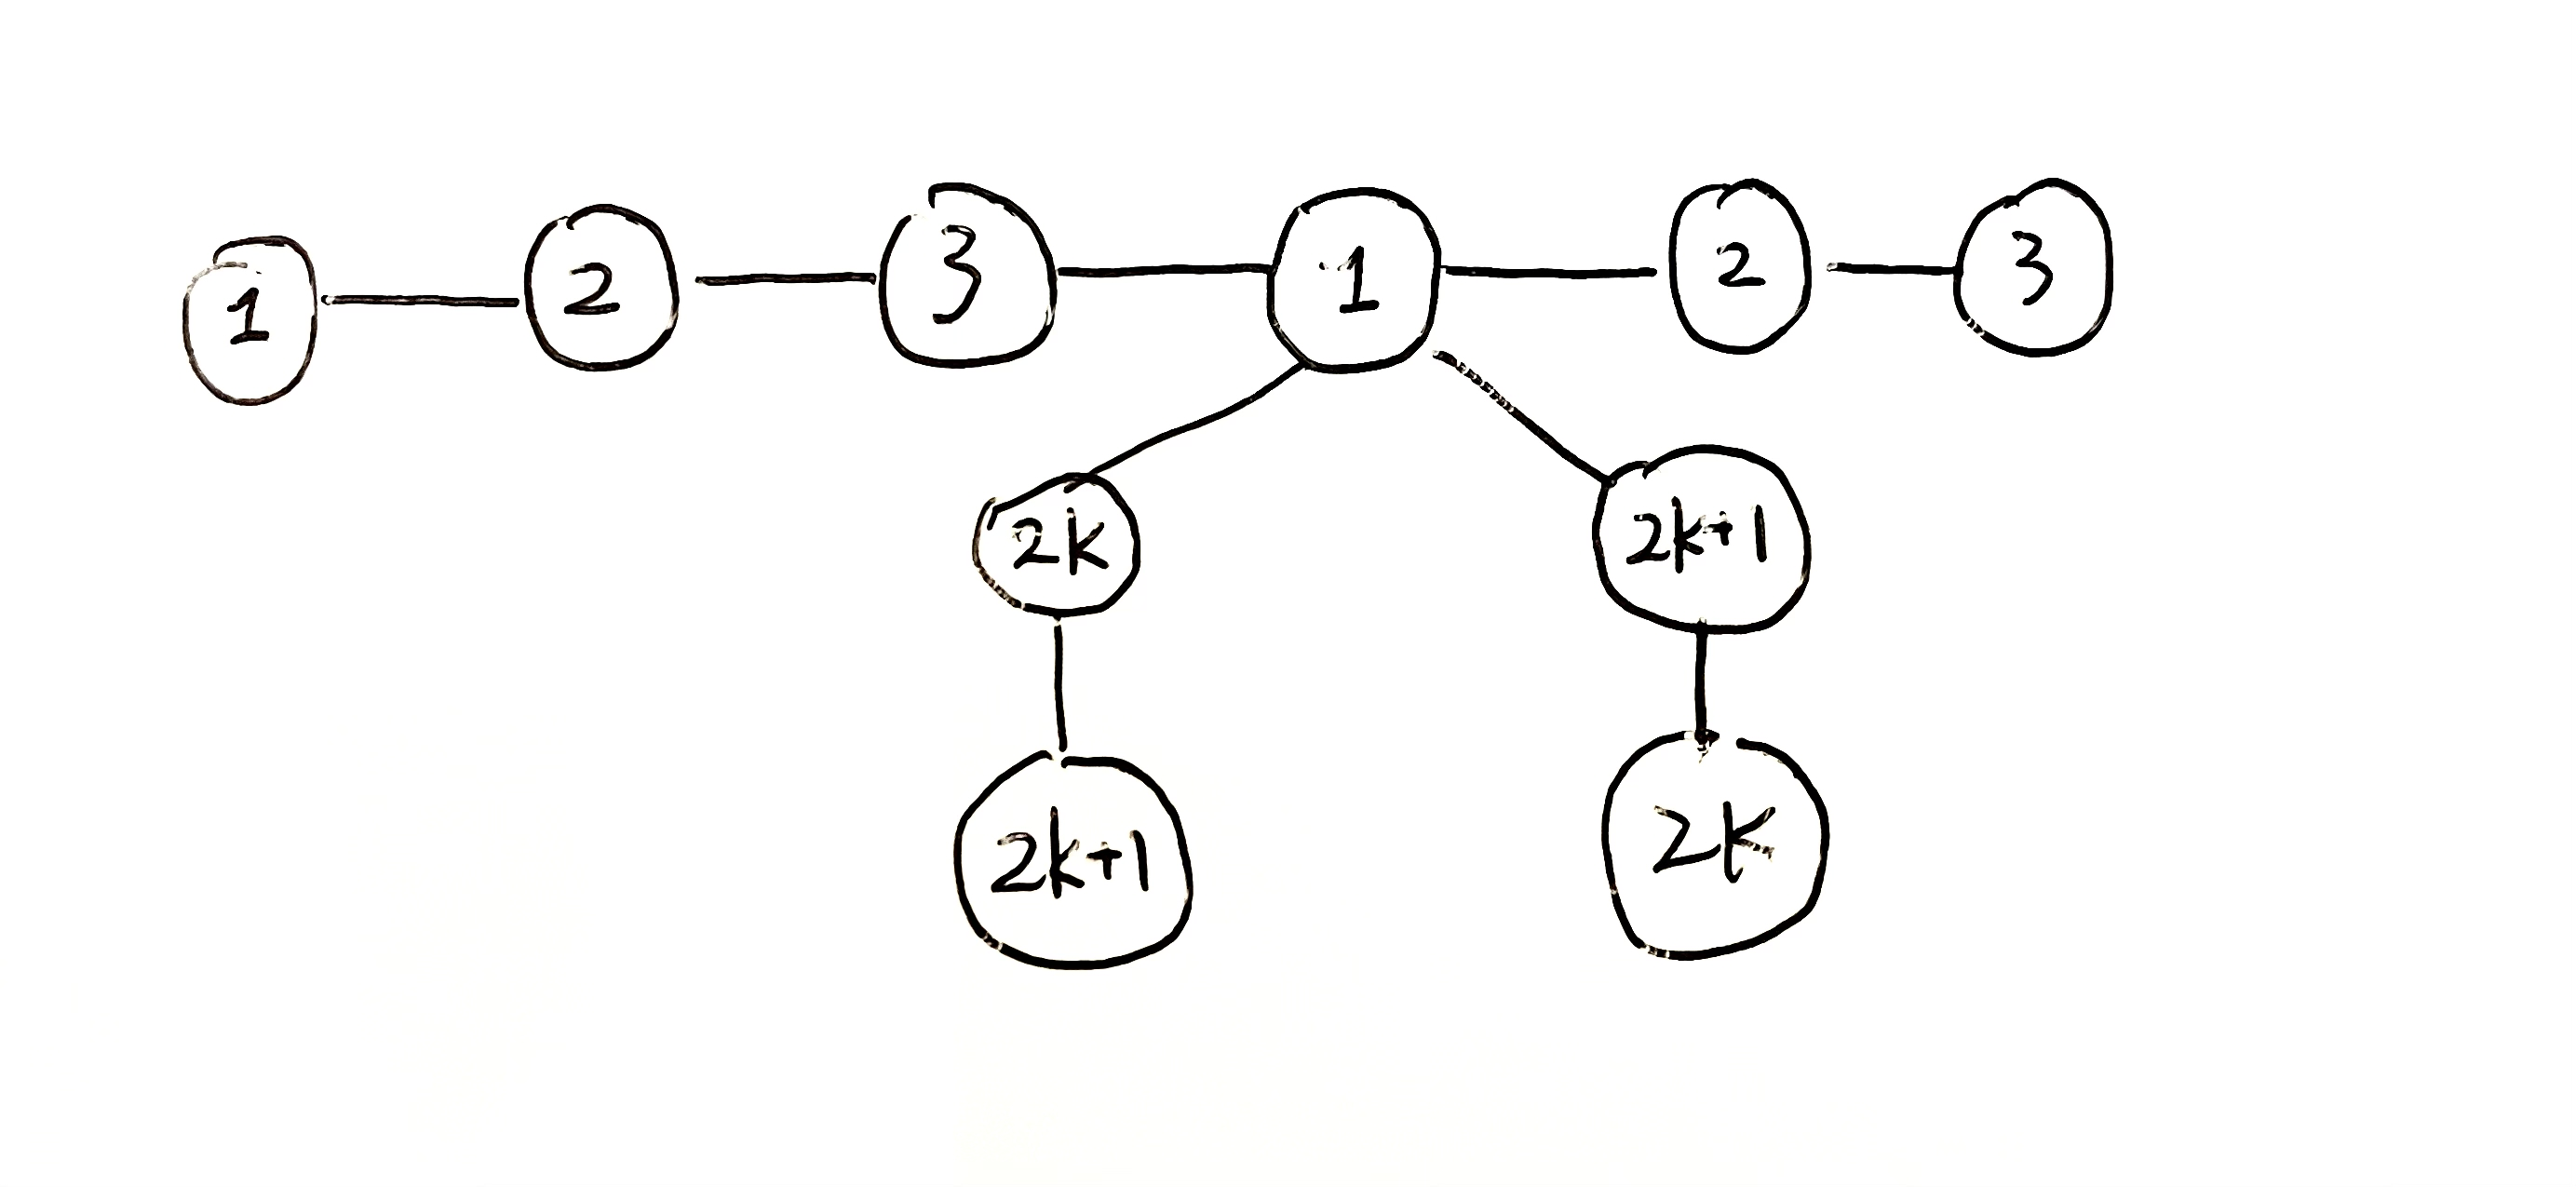
\includegraphics[width=0.7\textwidth]{solutions/img/agc035c/agc035c.jpg}
\end{center}

然后我们考虑 $n$ 是偶数的情况,我们考虑先构造出 $n-1$ 的答案,然后找到最大的 $m=2^k<n$,然后我们连接 $n\sim m\sim 1\sim (n-m+1)\sim n$ 即可。

关于 $n$ 是偶数的情况听了一下他的 tutorial,他大概是这样想的:因为 $1$ 连了 $2\sim n-1$ 的点,一个简单的思想是能不能找到 $n\sim a\sim 1\sim b\sim n$ 使得 $n\bigoplus a\bigoplus 1\bigoplus b\bigoplus n=n$,于是可以得到 $a\bigoplus b=n+1$,这时候想到 $m\bigoplus (n-m+1)=n+1$ 比较自然。

\ptitle{[AGC026F] Manju Game}{pufanyi}

\prob 有 $n$ 个箱子排成一列,第 $i$ 个箱子价值为 $a_i$。先手先随便选一个箱子并将其拿走。接着,两个人轮流操作,如果上一个人选的箱子为 $i$,那当前这个人只能选 $i-1$ 或者 $i+1$ 两个箱子中的其中一个。如果这两个箱子已经都被人拿走了或者不存在,那么这个人可以任意在这个序列中选择一个没被取过的箱子并且取走。如果两个人都是聪明的,他们都想得到箱子的价值和最大化,求最终先手和后手得到的价值。
\sol 假设所有奇数箱子的价值和为 $A$,偶数箱子的价值和为 $B$。

如果 $n$ 为偶数,摸一下不难发现答案为 $\left<\max\{A, B\}, \min\{A, B\}\right>$。

现在考虑 $n$ 为奇数的情况。我们分类讨论当前情况下先手选的是奇数箱子还是偶数箱子。偶数箱子比较好讨论,因为他把两边划分成了两段奇数箱子。这时候后手需要选一个方向进行取箱子。将这个方向的箱子取完后,我们发现留下了奇数个箱子,这时候当前的先手仍然是原来的先手,于是就变成了一个递归问题。

\begin{center}
    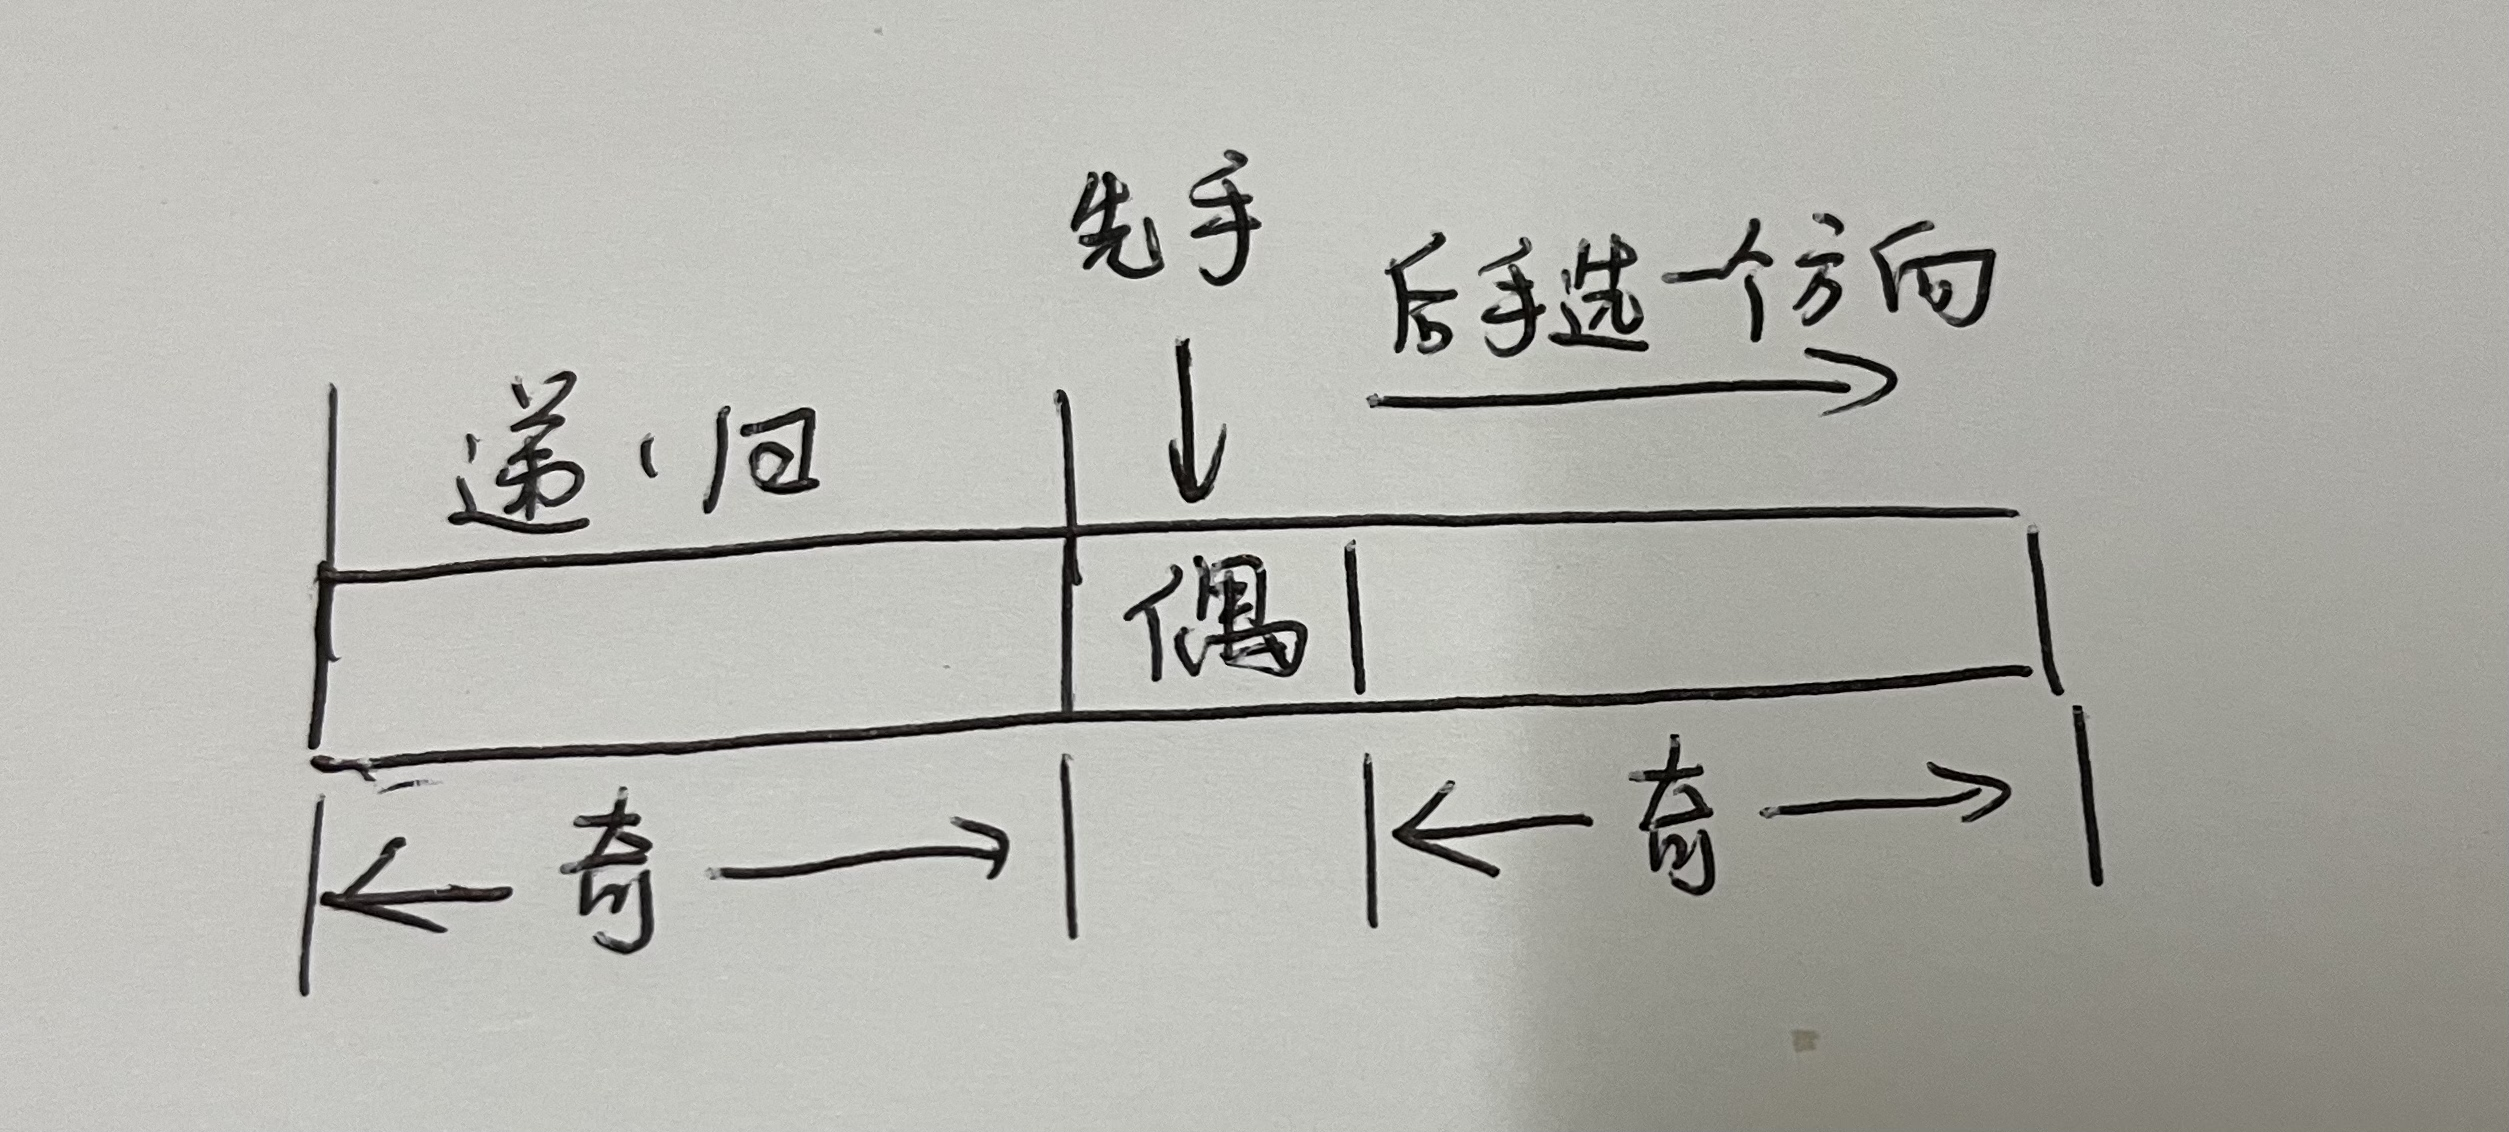
\includegraphics[width=0.5\textwidth]{solutions/img/agc026f/agc026f_1.jpg}
\end{center}

然后考虑取奇数的情况。首先我们发现一点,就是如果开局取奇数,先手得到的是一定不会小于 $A$ 的,因为我们可以 $1, 3, 5, \cdots$ 这样选。然后通过观察我们发现先手得到的也是不可能大于 $A$ 的,因为假设不这样选,先手一开始选了中间的一个 $k$,那么假设后手选择向右取完了 $k\sim n$,取完后我们发现对于 $1\sim k-1$,这一段区间中是原来的后手先选。这时候,后手完全可以 $k-1, k-3, k-5, \cdots$ 来强迫先手达到 $A$。而这只是一种方案,有可能有其他更有方案。因此,$1, 3, 5, \cdots$ 这样取就是最优的。

然后我们摸一下发现是这样的事情:首先先手选了一个偶数,后手选择一段,先手再选一个偶数,后手选择一段……直到某一时刻先手发现自己的最优策略就是把剩下所有的奇数箱子全部取完。这时候先手取完所有剩下的奇数,后手取完剩下的所有偶数,游戏结束。

仔细观察这个过程,我们发现相当于是先手每次选一个偶数点作为“关键点”,这时候后手选择这个关键点向左或向右将某一半的奇数点取走。经过这样的操作。我们发现以这些关键点分段,其实把整个序列分成了很多小的部分,而后手其实是选择了一个部分取走其中的偶数点,而取走其他部分的奇数点。(先手每次选择一个关键点,然后后手朝着离这个想选偶数点的区间的反方向将所有的奇数点取走)。

我们考虑二分答案 $x$,然后先手贪心地将每一段切的都满足这段中的奇数点权和减去偶数点权和小于等于 $x-B$。贪心复杂度 $\mathcal{O}(n)$。

故总复杂度 $\mathcal{O}(n\log\max\{a_i\})$。